\documentclass[12pt]{article}
\usepackage{geometry}
\usepackage{setspace}
\usepackage{graphicx}
\usepackage{booktabs}
\usepackage{float}
\usepackage[hidelinks]{hyperref}
\usepackage{amsmath}
\usepackage{amssymb}
\usepackage[utf8]{inputenc}
\usepackage{listings}
\usepackage{xcolor}
\usepackage{array}
\geometry{margin=1in}
\setstretch{1.15}

\lstset{
	language=Python,
	basicstyle=\ttfamily\footnotesize,
	backgroundcolor=\color{gray!10},
	frame=single,
	breaklines=true,
	breakatwhitespace=false,
	numbers=left,
	numberstyle=\tiny\color{gray},
	numbersep=5pt,
	showstringspaces=false,
	tabsize=4,
	captionpos=b,
	keywordstyle=\color{blue!70},
	stringstyle=\color{red!60},
	commentstyle=\color{green!50!black},
	morekeywords={as, True, False, None}
}

\title{\textbf{AAI 627 Homework 5\\ ROC Curves and Logistic Regression}}
\author{\textbf{Jude Eschete}}
\date{\today}

\begin{document}

	\maketitle
    \newpage
	%======================================================================
	\section{Part 1: Understanding the ROC Curve}
	%======================================================================

	\subsection{Problem Setup}

	Given the following logistic regression output probabilities and ground-truth class labels, the goal is to construct the ROC (Receiver Operating Characteristic) curve by computing the True Positive Rate (TPR) and False Positive Rate (FPR) at each possible classification threshold.

	\begin{align*}
		\textbf{Probabilities} &= [0.967,\ 0.448,\ 0.568,\ 0.879,\ 0.015,\ 0.780,\ 0.978,\ 0.004] \\
		\textbf{Classifications} &= [1,\ 0,\ 1,\ 0,\ 1,\ 0,\ 1,\ 0]
	\end{align*}

	There are $P = 4$ positive samples and $N = 4$ negative samples. The TPR and FPR are defined as:

	\begin{equation}
		\text{TPR} = \frac{TP}{TP + FN} = \frac{TP}{P}, \qquad
		\text{FPR} = \frac{FP}{FP + TN} = \frac{FP}{N}
	\end{equation}

	\subsection{Threshold Sweep}

	To construct the ROC curve, the samples are sorted by predicted probability in descending order. The classification threshold is swept from high to low; at each step the sample is predicted positive and the confusion matrix is updated accordingly.

	\begin{table}[H]
		\centering
		\caption{ROC curve computation: samples sorted by predicted probability (descending).}\label{tab:roc}
		\begin{tabular}{ccccccc}
			\toprule
			\textbf{Step} & \textbf{Probability} & \textbf{True Class} & \textbf{TP} & \textbf{FP} & \textbf{TPR} & \textbf{FPR} \\
			\midrule
			0 (start) & --- & --- & 0 & 0 & 0.00 & 0.00 \\
			1 & 0.978 & 1 & 1 & 0 & 0.25 & 0.00 \\
			2 & 0.967 & 1 & 2 & 0 & 0.50 & 0.00 \\
			3 & 0.879 & 0 & 2 & 1 & 0.50 & 0.25 \\
			4 & 0.780 & 0 & 2 & 2 & 0.50 & 0.50 \\
			5 & 0.568 & 1 & 3 & 2 & 0.75 & 0.50 \\
			6 & 0.448 & 0 & 3 & 3 & 0.75 & 0.75 \\
			7 & 0.015 & 1 & 4 & 3 & 1.00 & 0.75 \\
			8 & 0.004 & 0 & 4 & 4 & 1.00 & 1.00 \\
			\bottomrule
		\end{tabular}
	\end{table}

	\subsection{ROC Curve and AUC}

	The resulting ROC curve is plotted in Figure~\ref{fig:roc_part1}. The Area Under the Curve (AUC) is computed via the trapezoidal rule over the FPR axis:

	\begin{align*}
		\text{AUC} &= (0.25)(0.50 - 0.00)\cdot\tfrac{1}{1}
		             + (0.25)(0.50)\cdot 1
		             + (0.25)(0.75)\cdot 1
		             + (0.25)(1.00)\cdot 1 \\
		           &= 0.125 + 0.125 + 0.1875 + 0.25 \\
		           &= \boxed{0.6875}
	\end{align*}

	The AUC of 0.6875 indicates moderate discriminative ability - better than random (AUC = 0.5) but not yet a strong classifier (AUC = 1.0). Three of the four negatives received higher predicted probabilities than at least one positive, which pushes the curve below the ideal upper-left corner.

	\begin{figure}[H]
		\centering
		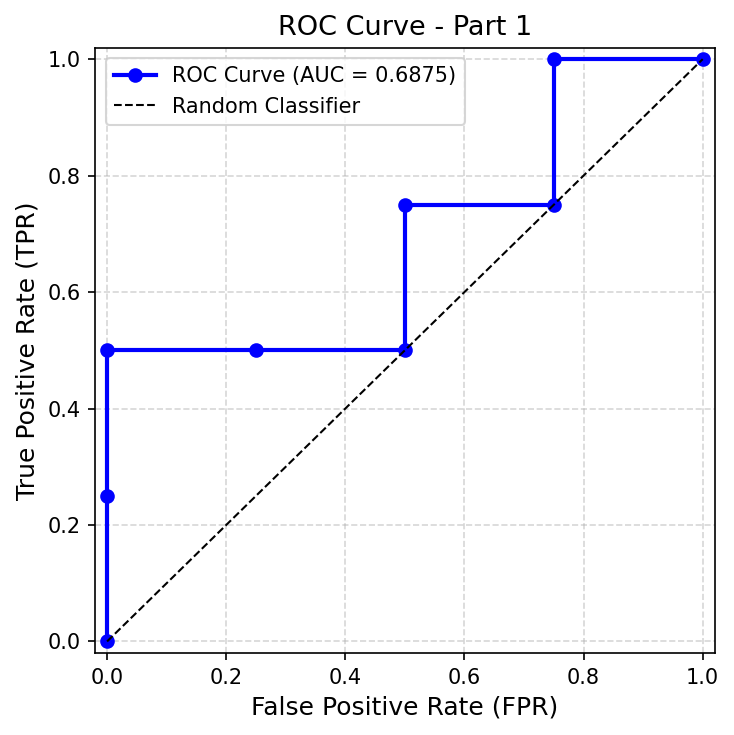
\includegraphics[width=0.6\textwidth]{roc_part1.png}
		\caption{ROC curve constructed from the given probabilities and ground-truth labels. The dashed diagonal represents a random classifier (AUC = 0.5). The computed AUC = 0.6875.}\label{fig:roc_part1}
	\end{figure}

	\newpage
	%======================================================================
	\section{Part 2: Logistic Regression on \texttt{dataSet\_1.mat}}
	%======================================================================

	\subsection{Dataset Overview}

	The dataset \texttt{dataSet\_1.mat} contains 4{,}000 samples and 476 features, with a binary response variable (2{,}362 positives and 1{,}638 negatives). The Python equivalents of the MATLAB functions used are:

	\begin{itemize}
		\item \texttt{glmfit} $\rightarrow$ \texttt{sklearn.linear\_model.LogisticRegression}
		\item \texttt{glmval} $\rightarrow$ \texttt{predict\_proba}
		\item \texttt{perfcurve} $\rightarrow$ \texttt{sklearn.metrics.roc\_curve} and \texttt{auc}
	\end{itemize}

	Features were standardized with \texttt{StandardScaler} (zero mean, unit variance) before fitting to ensure solver convergence with 476-dimensional input.

	%--------------------------------------------------
	\subsection{Task 1: Full-Dataset ROC Curve}
	%--------------------------------------------------

	Logistic regression was trained on all 4{,}000 samples. The predicted probabilities were then used to compute the ROC curve against the full response vector.

	\begin{center}
		\textbf{Full-Dataset AUC = 0.8426}
	\end{center}

	An AUC of 0.8426 indicates strong in-sample discriminative performance: the model ranks a randomly chosen positive above a randomly chosen negative about 84\% of the time.

	\begin{figure}[H]
		\centering
		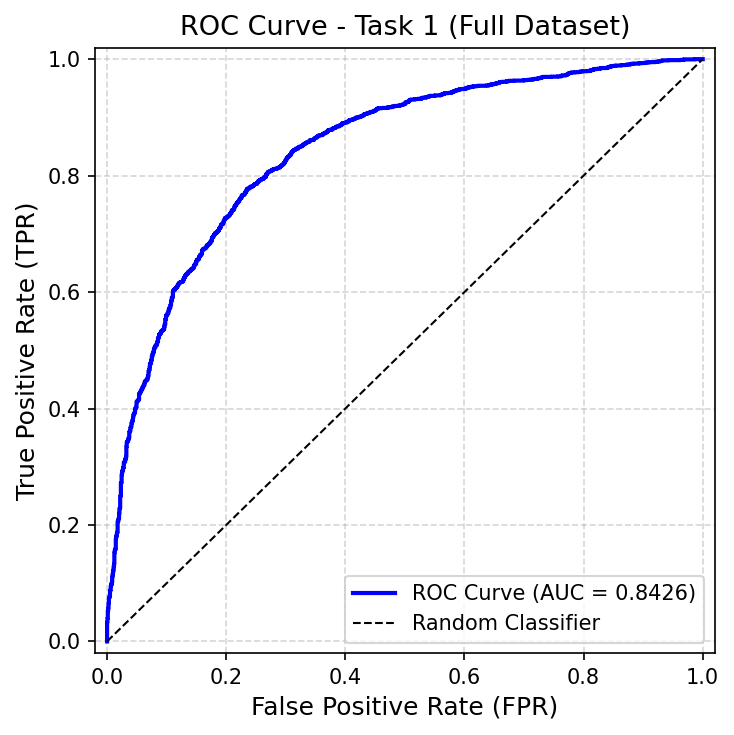
\includegraphics[width=0.6\textwidth]{roc_task1.png}
		\caption{ROC curve for Task 1 using the full dataset (4{,}000 samples, 476 features). AUC = 0.8426.}\label{fig:roc_task1}
	\end{figure}

	%--------------------------------------------------
	\subsection{Task 2: Train/Validation Split}
	%--------------------------------------------------

	The data were split as specified:
	\begin{itemize}
		\item \textbf{Training set:} rows 1--3{,}000 (3{,}000 samples)
		\item \textbf{Validation set:} rows 3{,}001--4{,}000 (1{,}000 samples)
	\end{itemize}

	The scaler and logistic regression model were fit exclusively on the training set. The trained model was then applied to both sets to generate predicted probabilities, from which separate ROC curves were computed.

	\begin{table}[H]
		\centering
		\caption{AUC comparison between training and validation sets.}\label{tab:auc_task2}
		\begin{tabular}{lc}
			\toprule
			\textbf{Dataset} & \textbf{AUC} \\
			\midrule
			Training   (rows 1--3{,}000)    & 0.8837 \\
			Validation (rows 3{,}001--4{,}000) & 0.4668 \\
			\midrule
			Difference & 0.4169 \\
			\bottomrule
		\end{tabular}
	\end{table}

	\begin{figure}[H]
		\centering
		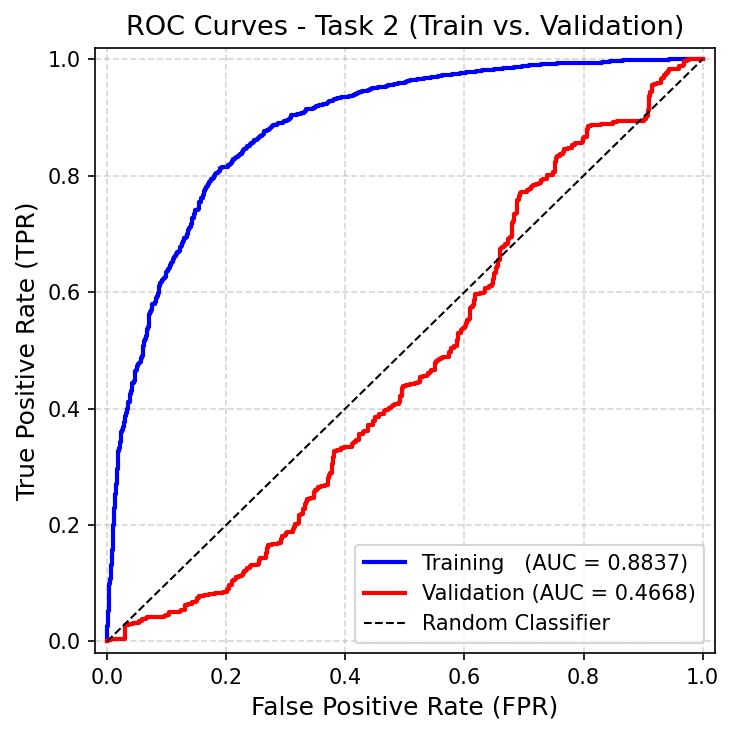
\includegraphics[width=0.6\textwidth]{roc_task2.png}
		\caption{ROC curves for Task 2. Blue: training set (AUC = 0.8837). Red: validation set (AUC = 0.4668). The large gap reveals severe overfitting.}\label{fig:roc_task2}
	\end{figure}

	\subsection{Discussion: Training vs.\ Validation AUC}

	The training AUC (0.8837) is substantially higher than the validation AUC (0.4668), a difference of 0.4169. A validation AUC below 0.5 is particularly notable: it means the model's probability rankings are \textit{inverted} relative to the true labels on held-out data -- the classifier is performing worse than random guessing on the validation set.

	This outcome is a textbook example of high-dimensional overfitting. With 476 features and only 3{,}000 training samples, the default L2-regularized logistic regression memorizes training-set patterns that do not generalize. The model effectively learns noise rather than signal, causing its predictions to be anti-correlated with the true validation labels.

	In practice, this would call for stronger regularization (lower \texttt{C}), dimensionality reduction (e.g., PCA), or feature selection before fitting the model.

	\newpage
	%======================================================================
	\section{Appendix: Python Code}
	%======================================================================

	\lstinputlisting[caption={AAI627\_HW5\_Eschete.py},label={lst:code}]{AAI627_HW5_Eschete.py}

\end{document}
